Este capítulo se centra en la fase de evaluación de los modelos entrenados y correspondiente con la penúltima fase de la metodología CRISP-DM. Se describe el conjunto de datos de prueba, el proceso de evaluación, la presentación de los resultados de las métricas y el análisis de las fortalezas y debilidades de los modelos.

\section{Conjunto de datos de prueba}
Para obtener el conjunto de datos para el entrenamiento de los modelos y el conjunto de datos de prueba, se ha de dividir el conjunto total de los datos, una vez que estos han sido preparados como siguiendo los pasos que se comentan en la sección anterior \ref{sec.prep-datos} \nameref{sec.prep-datos}. 


Al dividir el conjunto de datos, es crucial aplicar estratificación. Como se menciona en capítulos previos, esta técnica implica segmentar los datos de forma que se mantenga la misma distribución de clases en cada subconjunto. Esto resulta especialmente útil cuando las clases están desbalanceadas, ya que garantiza que todos los subconjuntos cuenten con una representación proporcional de cada clase, lo que mejora la precisión del modelo y minimiza los sesgos. Dado el desbalanceo observado en los datos de este trabajo, es esencial realizar una estratificación en cada división de los datos para evitar que algunas particiones contengan únicamente datos de una clase.


La división del conjunto de datos suele ser de en un 80\% para entrenamiento y un 20\% para evaluación, esta división se fundamenta en la necesidad de proporcionar suficiente cantidad de datos para que el modelo aprenda de manera efectiva, mientras se mantiene un conjunto de datos no utilizado en el entrenamiento para evaluar su rendimiento generalizando. La proporción del 80\% se considera adecuada para capturar patrones significativos en el entrenamiento sin comprometer la capacidad de evaluar el modelo en datos no vistos, lo que permite estimar su desempeño en situaciones realistas. Esta práctica también ayuda a evitar el sobreajuste, garantizando que los resultados del modelo no dependa en exclusiva de los datos utilizados en el entrenamiento \cite{bishop2006pattern}.

Para realizar la división, se utiliza la función \texttt{train\_test\_split} de la biblioteca \texttt{sklearn. model\_selection}. Esta función recibe el conjunto de los atributos y de las etiquetas de todo el \textit{dataset} utilizado, una vez que sus datos han sido preparados. Además, esta función recibe el porcentaje de los datos que se desea reservar para la evaluación o la fase de test, como se comenta en el párrafo anterior, en este trabajo el $0.2$ sobre 1 de los datos se destinan a evaluar los modelos entrenados. Finalmente, se especifica una semilla para que los datos se organicen de manera aleatoria y se especifica que se desea estratificar siguiendo el conjunto de las etiquetas.

Una vez divididos los datos, se normalizan los datos de evaluación, se convierten a tensores el conjunto de los atributos de pruebas y el conjunto de las etiquetas y se crea con estos tensores la instancia de la clase \texttt{DatasetTFG} que se utilizará para evaluar los modelos.

\section{Proceso de evaluación}
En el proceos de búsqueda de las configuraciones de hiperparámetros de los modelos con las que estos convergen mejor hacia una solución más generalizada, se ha utilizado la validación cruzada como se comenta en la Sección \ref{subsec:conjdatent}. La validación cruzada se utiliza para encontrar los mejores hiperparámetros de un modelo debido a su capacidad para proporcionar una evaluación más robusta y confiable del rendimiento del modelo. Este método divide el conjunto de datos en varios subconjuntos, realizando múltiples entrenamientos y evaluaciones, lo que permite reducir el riesgo de sobreajuste a un subconjunto específico. Además, la validación cruzada maximiza el uso de los datos disponibles, lo que resulta especialmente útil cuando los datos son limitados. 

Una vez que se han encontrado los hiperparámetros óptimos, se utiliza todo el conjunto de datos de entrenamiento, es decir, el 80\% del conjunto de datos para entrenar los modelos finales. Esto se debe a que, al haber ajustado previamente los hiperparámetros, se considera que los modelos se encuentran en sus configuraciones más eficientes, lo cual maximiza sus capacidades de generalización al aprender de la mayor cantidad de datos posible. De este modo, se obtienen unos modelos más robusto antes de realizar la evaluación final sobre un conjunto de prueba independiente que no ha sido utilizado en el proceso de entrenamiento \cite{hastie2009elements}.

El procesos de evaluación consiste en proporcionar a los modelos entrenados con las configuraciones comentadas en los párrafos anteriores, los datos de evaluación que no han visto durante la fase de entrenamiento. Durante este proceso se recogen los resultados que se obtienen en función de la matriz de confusión correspondiente a cada modelo para posteriormente obtener las métricas con las que comparar el desempeño de los modelos.

\section{Resultados de las métricas en el proceso de evaluación}
Para comparar los resultados obtenidos en la fase de evaluación de las cinco mejores configuraciones de hiperparámetros de cada arquitectura de cada modelo, se utilizan las mismas métricas comentadas en las secciones \ref{sec.metricas-bin} \nameref{sec.metricas-bin} y \ref{sec:metricas-mul} \nameref{sec:metricas-mul} correspondientemente.

Con el objetivo de que la interpretación de los datos sea más sencilla, se ha añadido a las siguientes figuras una columna con la posición del \textit{ranking} que ocupó cada configuración en la fase anterior.


\subsection{Resultados del modelo de clasificación binaria}
La métrica utilizada para establecer el orden en los siguientes \textit{rankings} de configuraciones para los modelos de clasificación binaria es la misma empleada durante la fase previa de búsqueda de las mejores configuraciones de hiperparámetros: el \textit{Recall}.

\subsubsection{MCB25: Modelo de clasifcación binaria con un tamaño de capa oculta igual a la mitad del número de atributos de entrada que recibe el modelo}
En la Tabla \ref{fig:EVALMCB25}, se muestran los resultados obtenidos durante las evaluaciones de las cinco configuraciones de hiperparámetros con mejor desempeño durante la fase de búsqueda mencionados en la Figura \ref{fig:BINhs25}. Corresponden con las mejores configuraciones para la arquitectura del modelo de clasificación binaria que posee un tamaño de capa oculta de 25 neuronas.

\begin{tabular}{|>{\columncolor[HTML]{E0FFFF}}l|c|c|c|c|c|}
\hline
Posicion\_EXP & 3º-BNC25 & 2º-BNC25 & 1º-BNC25 & 5º-BNC25 & 4º-BNC25 \\
\hline
\cellcolor[HTML]{E0FFFF}batch\_size & \cellcolor[HTML]{66ffa8}20000 & \cellcolor[HTML]{66ffa8}10000 & \cellcolor[HTML]{66ffa8}15000 & \cellcolor[HTML]{66ffa8}2000 & \cellcolor[HTML]{66ffa8}20000 \\
\cellcolor[HTML]{E0FFFF}learning\_rate & \cellcolor[HTML]{f99595}0.01 & \cellcolor[HTML]{f99595}0.001 & \cellcolor[HTML]{f99595}0.01 & \cellcolor[HTML]{f99595}0.001 & \cellcolor[HTML]{f99595}0.01 \\
\cellcolor[HTML]{E0FFFF}epochs & \cellcolor[HTML]{b1bafb}10 & \cellcolor[HTML]{b1bafb}30 & \cellcolor[HTML]{b1bafb}10 & \cellcolor[HTML]{b1bafb}10 & \cellcolor[HTML]{b1bafb}20 \\
\cellcolor[HTML]{E0FFFF}test\_recall & 0.998749 & 0.998640 & 0.998585 & 0.998422 & 0.998368 \\
\cellcolor[HTML]{E0FFFF}test\_accuracy & 0.999831 & 0.999813 & 0.999824 & 0.999826 & 0.999826 \\
\cellcolor[HTML]{E0FFFF}test\_f1 & 0.997934 & 0.997717 & 0.997853 & 0.997879 & 0.997879 \\
\cellcolor[HTML]{E0FFFF}test\_f2 & 0.998423 & 0.998271 & 0.998292 & 0.998205 & 0.998172 \\
\cellcolor[HTML]{E0FFFF}test\_precision & 0.997121 & 0.996796 & 0.997121 & 0.997337 & 0.997391 \\
\cellcolor[HTML]{E0FFFF}test\_roc\_auc & 0.999765 & 0.999772 & 0.999841 & 0.999818 & 0.999899 \\
\cellcolor[HTML]{E0FFFF}test\_specificity & 0.999877 & 0.999863 & 0.999877 & 0.999886 & 0.999888 \\
\hline
    %\caption{Resultados de la evaluación del modelo de  clasificación binaria con \textit{n/2} neuronas en la capa oculta siendo \textit{n} el número de atributos de entrada.}
    \label{fig:EVALMCB25}
\end{tabular}


Los valores de la métrica \textit{Recall} obtenidos en las evaluaciones del modelo MCB25, son muy altos para todas las configuraciones y la diferencia entre sus valores es del orden de $1*10^{-4}$. Estas diferencias pueden deberse a circunstancias no controlables como el estado en el que se encontraba la máquina cuando se realizó la evaluación de los modelos o los pesos aleatorios iniciales que se eligieron en esa ejecución de los test.

La matriz de confusión de la mejor configuración de hiperparámetros obtenida en el 3º MCB25 durante su evaluación es la que se muestra en la Figura \ref{fig:MC_EVAL_MCB25}.

\begin{figure}[H]
    \centering
    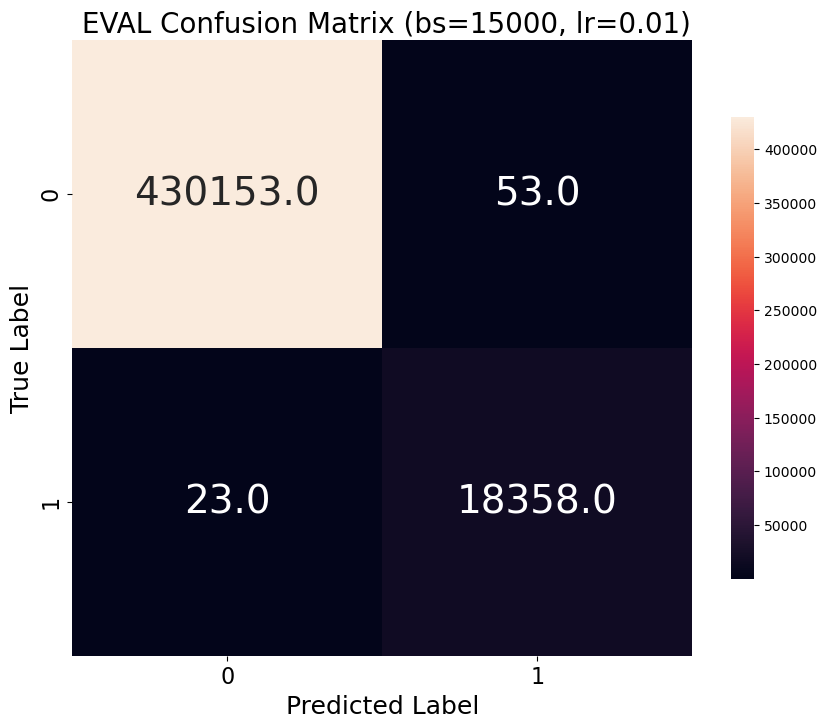
\includegraphics[width=0.5\textwidth]{./img/evaluacion/matrices_confusion/MC_EVAL_MCB25.png}
    \caption{Matriz de confusión de la mejor configuración de hiperparámetros obtenida en el 3º MCB25 durante la fase de evaluación.}
    \label{fig:MC_EVAL_MCB25}
\end{figure}


\subsubsection{MCB49: Modelo de clasifcación binaria con un tamaño de capa oculta igual al número de atributos de entrada que recibe el modelo}
En la Figura \ref{fig:EVALMCB49} se presentan los resultados obtenidos durante las evaluaciones de las cinco configuraciones de hiperparámetros con mejor desempeño, seleccionadas en la fase de búsqueda en la Figura \ref{fig:BINhs49} para la arquitectura del modelo de clasificación binaria que cuenta con una capa oculta de 49 neuronas.

\begin{figure}[H]
    \centering
    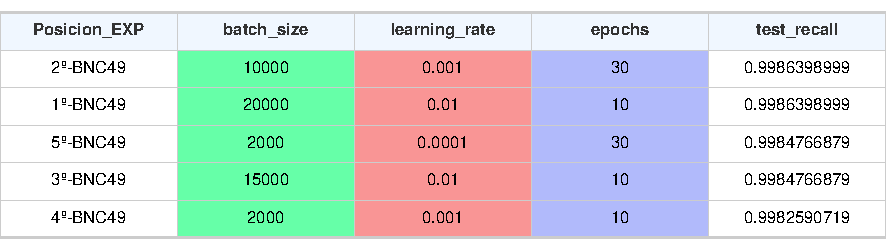
\includegraphics[width=0.9\textwidth]{./img/evaluacion/resultados/EVALMCB49.pdf}
    \caption{Resultados de la evaluación del modelo de clasificación binaria con \textit{n} neuronas en la capa oculta siendo \textit{n} el número de atributos de entrada.}
    \label{fig:EVALMCB49}
\end{figure}

Los valores de la métrica \textit{Recall} obtenidos durante las evaluaciones del modelo MCB49 son consistentemente altos para todas las configuraciones, y las diferencias entre ellos se encuentran en el orden de magnitud de $1*10^{-4}$. Estas variaciones podrían atribuirse a factores no controlables, como el estado del sistema al momento de la evaluación o la aleatoriedad en la inicialización de los pesos durante la ejecución de las pruebas.

La matriz de confusión correspondiente a la mejor configuración de hiperparámetros obtenida en el 2º MCB49 durante su evaluación se presenta en la Figura \ref{fig:MC_EVAL_MCB49}.

\begin{figure}[H]
    \centering
    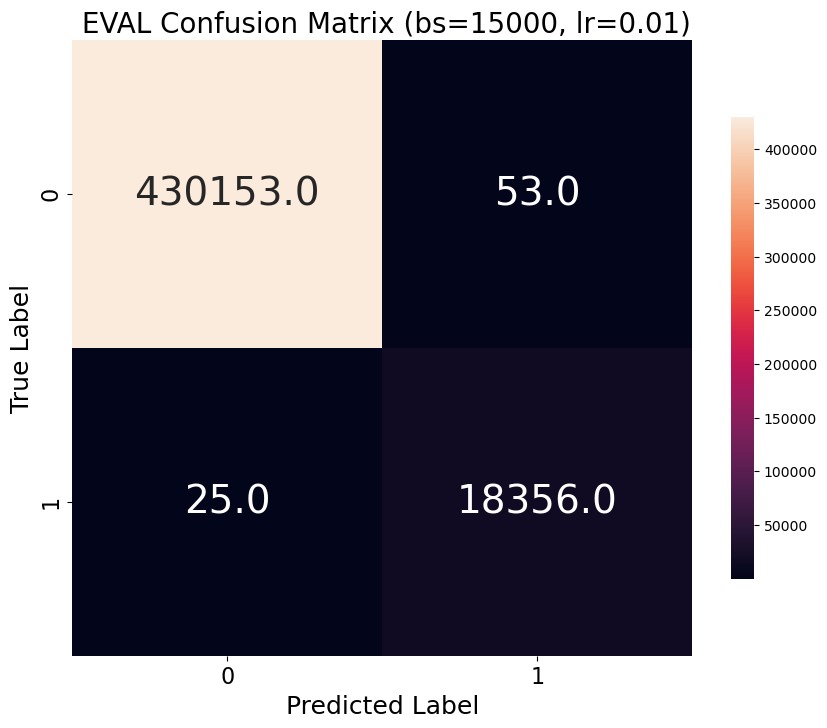
\includegraphics[width=0.5\textwidth]{./img/evaluacion/matrices_confusion/MC_EVAL_MCB49.png}
    \caption{Matriz de confusión de la mejor configuración de hiperparámetros obtenida en el 2º MCB49 durante la fase de evaluación.}
    \label{fig:MC_EVAL_MCB49}
\end{figure}



\subsubsection{MCB98: Modelo de clasifcación binaria con un tamaño de capa oculta igual al doble del número de atributos de entrada que recibe el modelo}
La Figura \ref{fig:EVALMCB98} muestra los resultados obtenidos en las evaluaciones correspondientes a las cinco configuraciones de hiperparámetros que presentaron el mejor desempeño durante la fase de búsqueda mostradas en al Figura \ref{fig:BINhs98}, aplicadas a la arquitectura del modelo de clasificación binaria con una capa oculta de 98 neuronas.

\begin{figure}[H]
    \centering
    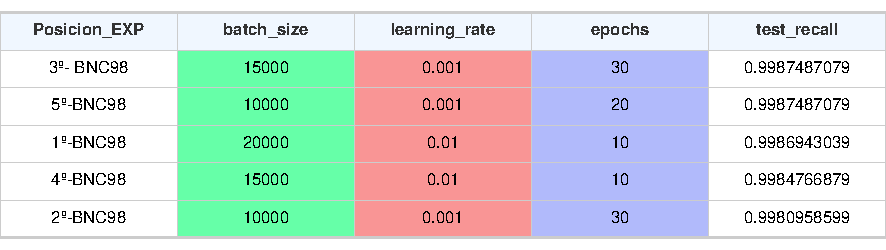
\includegraphics[width=0.9\textwidth]{./img/evaluacion/resultados/EVALMCB98.pdf}
    \caption{Resultados de la evaluación del modelo de clasificación binaria con \textit{2n} neuronas en la capa oculta siendo \textit{n} el número de atributos de entrada.}
    \label{fig:EVALMCB98}
\end{figure}

En las evaluaciones del modelo MCB98, los valores obtenidos para la métrica \textit{Recall} fueron elevados en todas las configuraciones, con diferencias del orden de $1*10^{-4}$. Estas pequeñas variaciones pueden explicarse por factores no controlables, como el estado del sistema en el momento de la evaluación o la inicialización aleatoria de los pesos durante la ejecución de las pruebas.


La matriz de confusión correspondiente a la mejor configuración de hiperparámetros obtenida en el 3º MCB98 durante su evaluación se presenta en la Figura \ref{fig:MC_EVAL_MCB98}.

\begin{figure}[H]
    \centering
    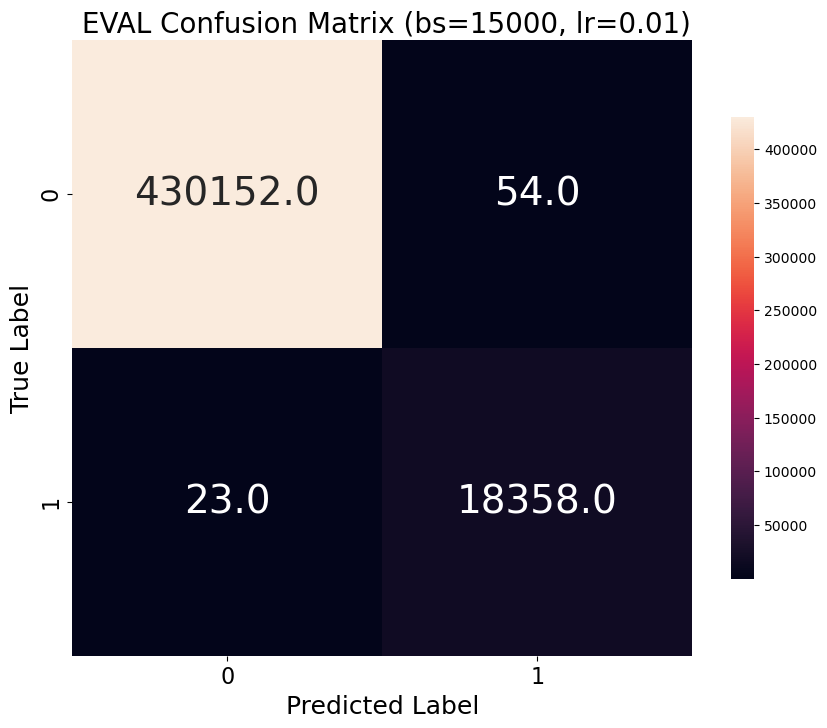
\includegraphics[width=0.5\textwidth]{./img/evaluacion/matrices_confusion/MC_EVAL_MCB98.png}
    \caption{Matriz de confusión de la mejor configuración de hiperparámetros obtenida en el 3º MCB98 durante la fase de evaluación.}
    \label{fig:MC_EVAL_MCB98}
\end{figure}




\subsection{Resultados del modelo de clasificación multiclase}
Para determinar el orden de los \textit{rankings} presentados a continuación, se emplea la misma métrica utilizada en la fase de búsqueda de configuraciones de hiperparámetros para los modelos de clasificación multiclase: el \textit{F1-weighted}.

\subsubsection{MCM25: Modelo de clasifcación multiclase con un tamaño de capa oculta igual a la mitad del número de atributos de entrada que recibe el modelo}

En la Figura \ref{fig:EVALMCM25} se presentan los resultados obtenidos durante las evaluaciones de las cinco configuraciones de hiperparámetros con mejores métricas, identificadas durante la fase de búsqueda de hiperparámetros para la arquitectura del modelo de clasificación multiclase que cuenta con una capa oculta de 25 neuronas.

\begin{figure}[H]
    \centering
    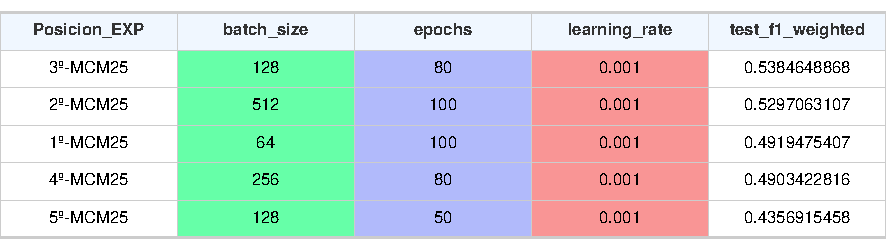
\includegraphics[width=0.9\textwidth]{./img/evaluacion/resultados/EVALMCM25.pdf}
    \caption{Resultados de la evaluación del modelo de clasificación multiclase con \textit{n/2} neuronas en la capa oculta siendo \textit{n} el número de atributos de entrada.}
    \label{fig:EVALMCM25}
\end{figure}

La figura anterior evidencia una diferencia en los valores de la métrica de comparación considerablemente mayor que la observada para las mismas configuraciones durante la fase de búsqueda de hiperparámetros. En los cinco mejores modelos representados en la figura, las diferencias en la métrica \textit{F1-weighted} durante la fase de búsqueda se encuentran en el orden de $1*10^{-2}$, mientras que en la fase de evaluación alcanzan un orden de $1*10^{-1}$, lo que indica una discrepancias con respecto a los resultados observados en la búsqueda de hiperparáemtros de la fase de modelado.

La matriz de confusión de la mejor configuración de hiperparámetros obtenida en el 3º MCM25 durante su evaluación, es la que se muestra en la Figura \ref{fig:MC_EVAL_MCM25}.

\begin{figure}[H]
    \centering
    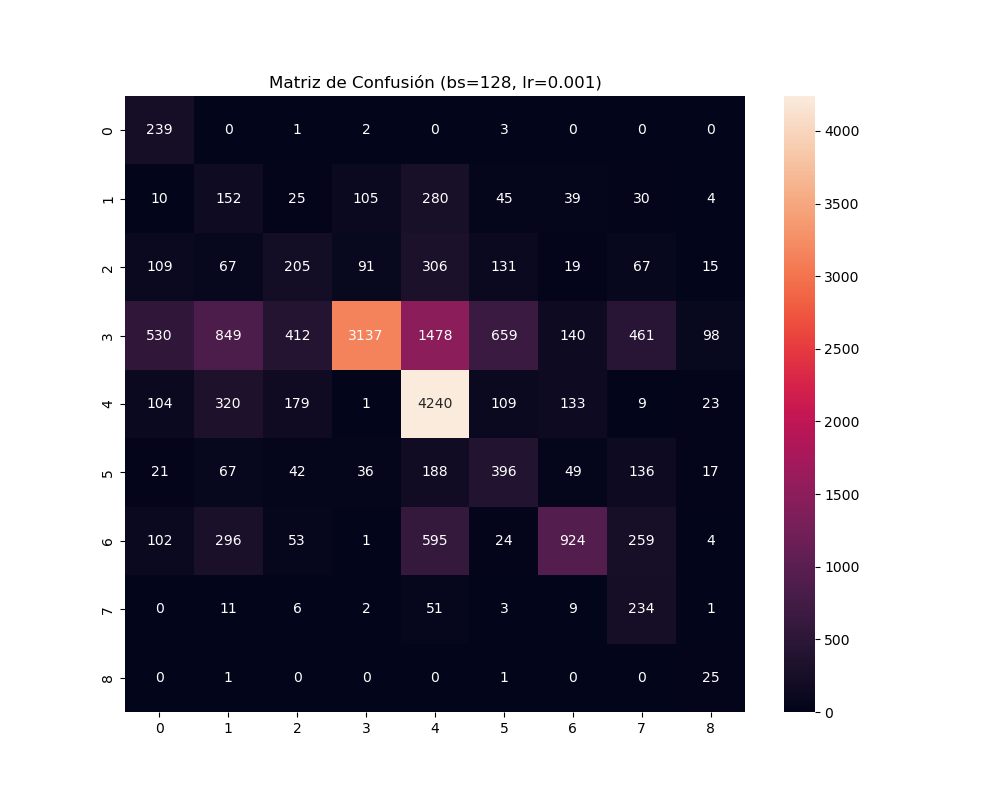
\includegraphics[width=0.8\textwidth]{./img/evaluacion/matrices_confusion/MC_EVAL_MCM25.png}
    \caption{Matriz de confusión de la mejor configuración de hiperparámetros obtenida con en el 3º MCM25 durante la fase de evaluación.}
    \label{fig:MC_EVAL_MCM25}
\end{figure}

Dado que los datos empleados para entrenar el modelo de clasificación multiclase presentan un elevado desbalance entre clases, se recurre a la funcionalidad de normalización de matrices de confusión de \texttt{wandb} para generar una representación visual más informativa que la mostrada en la Figura \ref{fig:MC_EVAL_MCM25}. Esta técnica permite observar de forma más clara el comportamiento del modelo en cada clase, independientemente de su frecuencia en los datos, tal y como se puede apreciar en la Figura \ref{fig:MCNorm_EVAL_MCM25}.

La normalización en \texttt{wandb} convierte los conteos absolutos de la matriz de confusión en proporciones por clase real, lo que facilita la comparación del rendimiento del modelo entre clases desbalanceadas.

\begin{figure}[H]
    \centering
    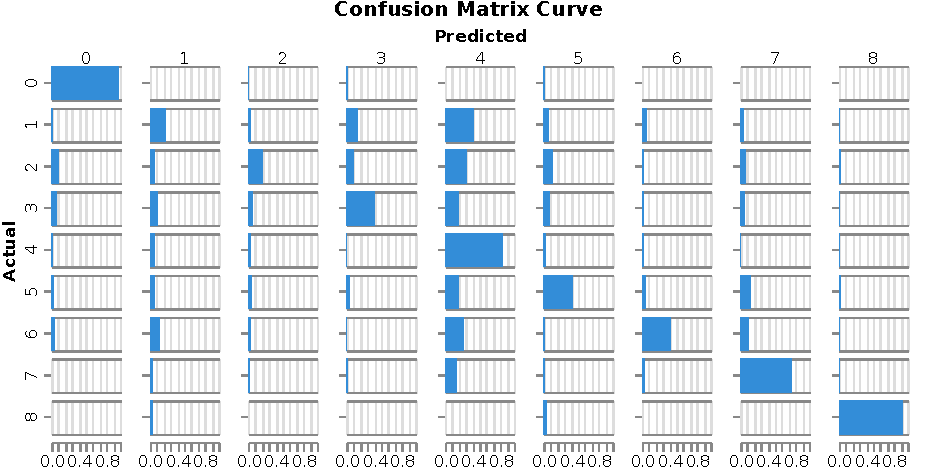
\includegraphics[width=0.95\textwidth]{./img/evaluacion/matrices_confusion/MCNorm_EVAL_MCM25.pdf}
    \caption{Matriz de confusión normalizada de la mejor configuración de hiperparámetros obtenida en el 3º MCM25 durante la fase de evaluación.}
    \label{fig:MCNorm_EVAL_MCM25}
\end{figure}



\subsubsection{MCB49: Modelo de clasifcación multiclase con un tamaño de capa oculta igual al número de atributos de entrada que recibe el modelo}
La Figura \ref{fig:EVALMCM49} presenta los resultados de las evaluaciones realizadas sobre las cinco configuraciones de hiperparámetros con mejores métricas, seleccionadas durante la fase de búsqueda aplicada a la arquitectura del modelo de clasificación multiclase con una capa oculta compuesta por 49 neuronas.

\begin{figure}[H]
    \centering
    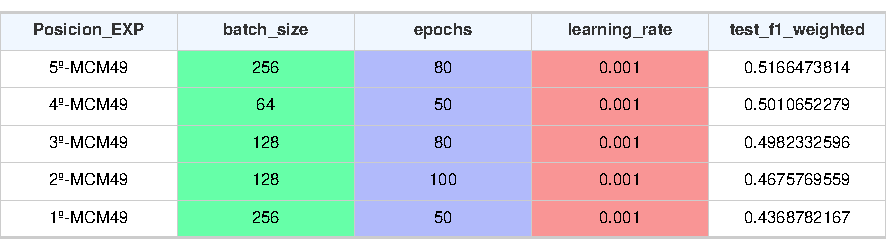
\includegraphics[width=0.9\textwidth]{./img/evaluacion/resultados/EVALMCM49.pdf}
    \caption{Resultados de la evaluación del modelo de clasificación multiclase con \textit{n} neuronas en la capa oculta siendo \textit{n} el número de atributos de entrada.}
    \label{fig:EVALMCM49}
\end{figure}

Al analizar los resultados obtenidos para esta arquitectura, destaca más allá del bajo rendimiento reflejado por la métrica \textit{F1-weighted}, el hecho de que el orden de las configuraciones se ha invertido respecto a lo observado en la fase de búsqueda. Las posibles causas de este comportamiento se detallan en la sección \ref{sec:analEVAL}.

La matriz de confusión de la mejor configuración de hiperparámetros obtenida en el 5º MCM49 durante su evaluación, es la que se muestra en la Figura \ref{fig:MC_EVAL_MCM49}.

\begin{figure}[H]
    \centering
    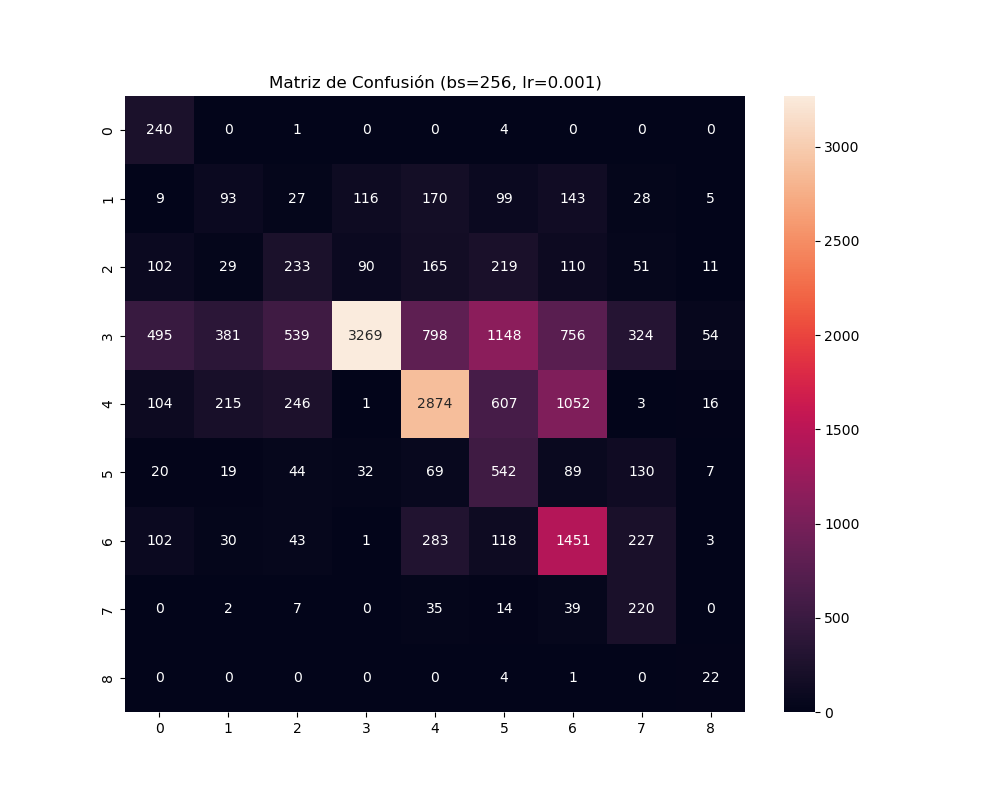
\includegraphics[width=0.8\textwidth]{./img/evaluacion/matrices_confusion/MC_EVAL_MCM49.png}
    \caption{Matriz de confusión de la mejor configuración de hiperparámetros obtenida con en el 5º MCM49 durante la fase de evaluación.}
    \label{fig:MC_EVAL_MCM49}
\end{figure}

Dado el elevado desbalance entre clases en los datos utilizados para entrenar el modelo de clasificación multiclase, se emplea la funcionalidad de normalización de matrices de confusión de \texttt{wandb} para generar una representación visual más informativa que la presentada en la Figura \ref{fig:MC_EVAL_MCM49}. Esta técnica facilita la observación más clara del comportamiento del modelo en cada clase, independientemente de su frecuencia en los datos, como se puede observar en la Figura \ref{fig:MCNorm_EVAL_MCM49}.

La normalización en \texttt{wandb} convierte los conteos absolutos de la matriz de confusión en proporciones por clase real, lo que facilita la comparación del rendimiento del modelo entre clases desbalanceadas.

\begin{figure}[H]
    \centering
    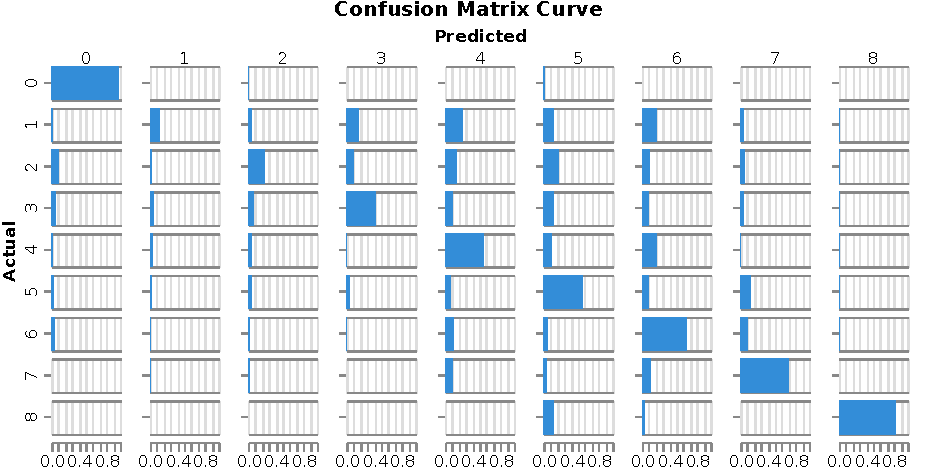
\includegraphics[width=0.95\textwidth]{./img/evaluacion/matrices_confusion/MCNorm_EVAL_MCM49.pdf}
    \caption{Matriz de confusión normalizada de la mejor configuración de hiperparámetros obtenida en el 5º MCM49 durante la fase de evaluación.}
    \label{fig:MCNorm_EVAL_MCM49}
\end{figure}




\subsubsection{MCB98: Modelo de clasifcación multiclase con un tamaño de capa oculta igual al doble del número de atributos de entrada que recibe el modelo}
En la Figura \ref{fig:EVALMCM98} se ilustran los resultados obtenidos durante las evaluaciones correspondientes a las cinco configuraciones de hiperparámetros con mejores métricas, seleccionadas en la etapa de búsqueda de configuraciones para la arquitectura del modelo de clasificación multiclase con una capa oculta de 98 neuronas..

\begin{figure}[H]
    \centering
    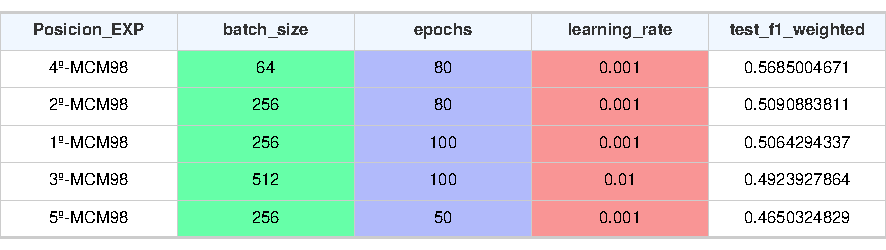
\includegraphics[width=0.9\textwidth]{./img/evaluacion/resultados/EVALMCM98.pdf}
    \caption{Resultados de la evaluación del modelo de clasificación multiclase con \textit{2n} neuronas en la capa oculta siendo \textit{n} el número de atributos de entrada.}
    \label{fig:EVALMCM98}
\end{figure}

Los resultados obtenidos durante la fase de evaluación de esta arquitectura fueron significativamente inferiores a los alcanzados en la fase de búsqueda. Por ejemplo, en la quinta mejor configuración de hiperparámetros, la diferencia entre los resultados experimentales y los obtenidos en la evaluación es del orden de $1*10^{-1}$. Esta diferencia implica una reducción del 10\% en la precisión, o bien, un mayor número de errores en las clases con menor cantidad de muestras en comparación con la fase anterior.


La matriz de confusión de la mejor configuración de hiperparámetros obtenida en el 4º MCM98 durante su evaluación, es la que se muestra en la Figura \ref{fig:MC_EVAL_MCM98}.

\begin{figure}[H]
    \centering
    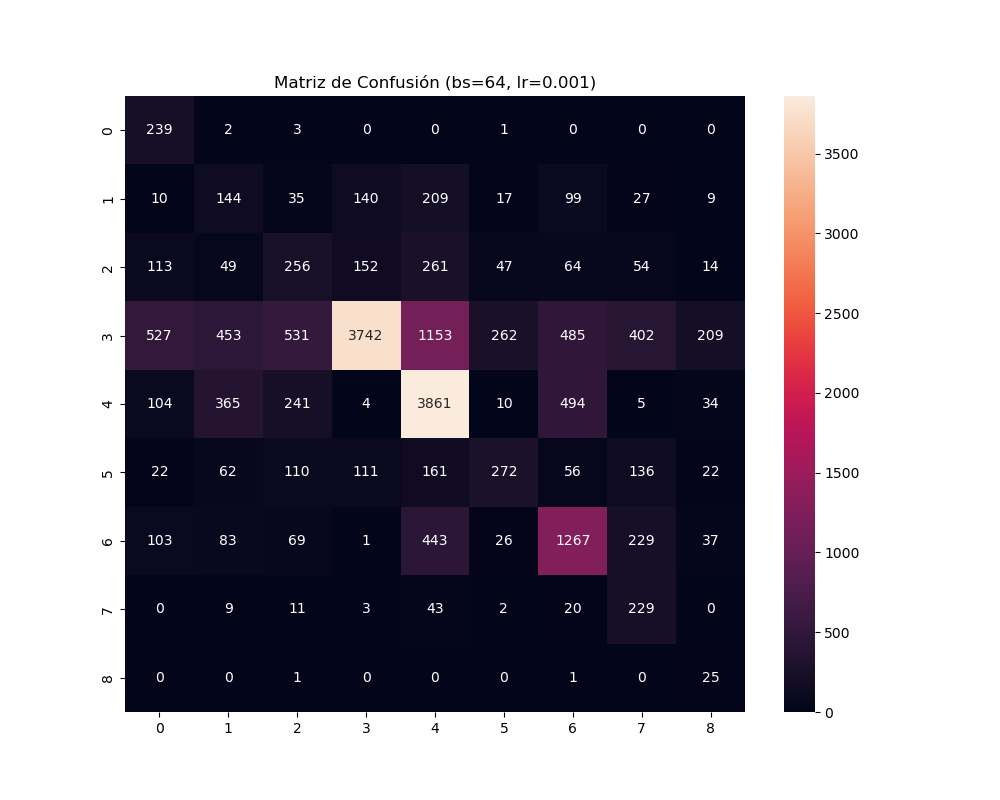
\includegraphics[width=0.8\textwidth]{./img/evaluacion/matrices_confusion/MC_EVAL_MCM98.png}
    \caption{Matriz de confusión de la mejor configuración de hiperparámetros obtenida en el 4º MCM98 durante la fase de evaluación.}
    \label{fig:MC_EVAL_MCM98}
\end{figure}

Debido al elevado desbalance entre clases en los datos utilizados para entrenar el modelo de clasificación multiclase, se recurre a la funcionalidad de normalización de matrices de confusión de \texttt{wandb}, con el fin de generar una representación visual más clara que la mostrada en la Figura \ref{fig:MC_EVAL_MCM98}. Esta técnica permite analizar de manera más precisa el comportamiento del modelo en cada clase, sin depender de su frecuencia en los datos, como se observa en la Figura \ref{fig:MCNorm_EVAL_MCM98}.

La normalización en \texttt{wandb} convierte los conteos absolutos de la matriz de confusión en proporciones por clase real, lo que facilita la comparación del rendimiento del modelo entre clases desbalanceadas.

\begin{figure}[H]
    \centering
    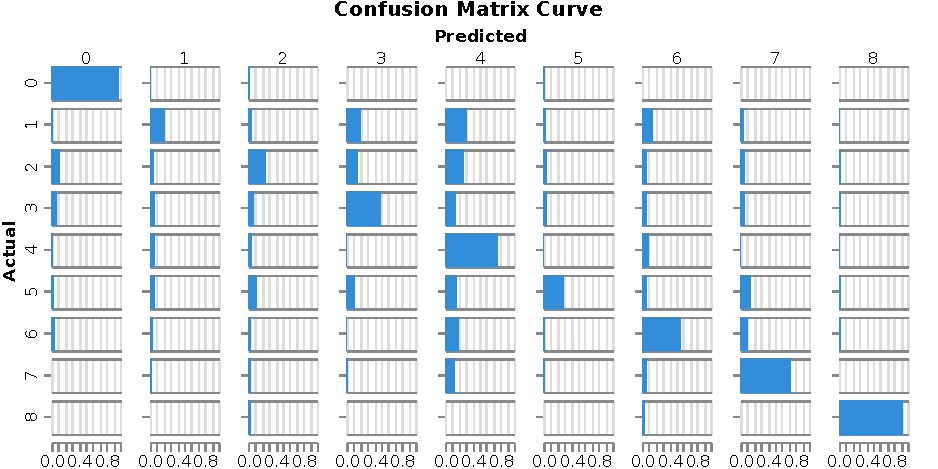
\includegraphics[width=0.85\textwidth]{./img/evaluacion/matrices_confusion/MCNorm_EVAL_MCM98.pdf}
    \caption{Matriz de confusión normalizada de la mejor configuración de hiperparámetros obtenida en el MCM98 durante la fase de evaluación.}
    \label{fig:MCNorm_EVAL_MCM98}
\end{figure}




\section{Análisis de los resultados obtenidos} \label{sec:analEVAL}
\subsection{Modelo de clasificación binaria}

Los resultados obtenidos durante la fase de búsqueda de las mejores configuraciones de hiperparámetros empleando validación cruzada \textit{k-fold} con estratificación muestran valores de \textit{Recall} consistentemente altos, todos por encima de $0{.}9985$, como se detalla en la Figura \ref{fig:BINtop5}. Este rendimiento indica una capacidad del modelo para identificar correctamente la clase mayoritaria de forma fiable y robusta en distintos subconjuntos de datos, lo cual respalda la estabilidad de las configuraciones seleccionadas durante esta fase de optimización \cite{bergstra2012random}.

Sin embargo, al aplicar estas mismas configuraciones en la fase de evaluación sobre un conjunto independiente (Figura \ref{fig:top5EVALMCB}), se observa una inversión parcial en el orden del rendimiento de las configuraciones. Algunas de las configuraciones con las mejores métricas en la búsqueda no mantienen su posición, mientras que otras ascienden en el \textit{ranking}. Este comportamiento puede atribuirse a pequeñas variaciones aleatorias en los datos o a la sensibilidad del modelo frente a distribuciones ligeramente diferentes, aun cuando estas diferencias se hayan mitigado mediante estratificación \cite{reimers2017optimal}.

A pesar de que las diferencias absolutas entre los valores de \textit{Recall} en ambas fases son reducidas (del orden de $1*10^{-4}$ a $1*10^{-3}$), su impacto puede ser relevante en tareas de clasificación binaria crítica, como la detección de conexiones maliciosas, donde incluso mínimas variaciones pueden traducirse en decisiones erróneas. El empeoramiento de algunas de las métricas puede deberse a factores como la inicialización aleatoria de pesos o el estado del sistema durante la inferencia, más que a un verdadero sobreajuste, dado que el proceso de validación cruzada ya controla adecuadamente este riesgo \cite{goodfellow2016deep}.

Asimismo, el análisis muestra que distintas combinaciones de \texttt{batch\_size}, \texttt{epochs}, \texttt{hidden \_size} y \texttt{learning\_rate} conducen a valores de \textit{Recall} muy próximos en evaluación. Esta convergencia en el rendimiento es coherente con estudios que sugieren que múltiples configuraciones en regiones planas del espacio de pérdida pueden llevar a modelos igualmente eficaces, especialmente en arquitecturas con un número de neuronal elevado como las utilizadas \cite{bouthillier2021sloppy}.

La observación de que varias configuraciones producen valores prácticamente idénticos de \textit{Recall} en la evaluación sugiere la presencia de una región de estabilidad en el espacio de soluciones. Sin embargo, el hecho de que estas configuraciones no coincidan con las mejor posicionadas en la búsqueda indica que, aunque la validación cruzada estratificada proporciona una estimación robusta, puede no capturar completamente la variabilidad inherente del conjunto de evaluación, especialmente si este presenta ligeras desviaciones de la distribución global \cite{recht2019imagenet}.

Los resultados reflejan un comportamiento coherente con lo esperado para modelos que han sido correctamente validados. Las diferencias encontradas entre fases no parecen ser estadísticamente significativas, pero sí lo suficientemente marcadas como para sugerir la conveniencia de utilizar estrategias complementarias de evaluación en futuros experimentos, como pruebas de sensibilidad o análisis de varianza.

\begin{figure}[H]
    \centering
    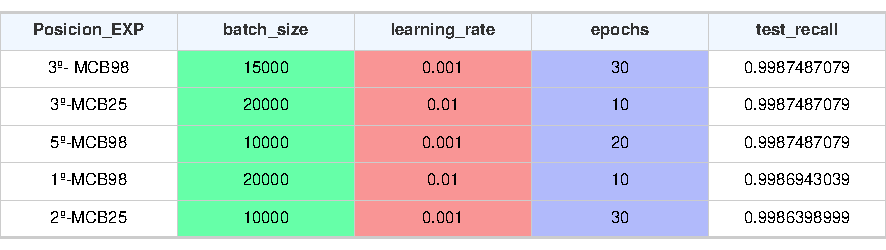
\includegraphics[width=0.9\textwidth]{./img/evaluacion/resultados/top5EVALMCB.pdf}
    \caption{Mejores cinco modelos en la fase de evaluación del modelo de clasificación binaria.}
    \label{fig:top5EVALMCB}
\end{figure}

\subsection{Modelo de clasificación multiclase}

Los resultados obtenidos durante la fase de búsqueda de hiperparámetros del modelo de clasificación multiclase (MCM), reflejados en la Figura \ref{fig:MULtop10}, indican valores moderados en las métricas utilizadas. En particular, el valor promedio de \textit{F1-weighted} se sitúa en torno a $0{.}57$, con ligeras variaciones entre las distintas configuraciones probadas. Este nivel de desempeño es coherente con la naturaleza desbalanceada del conjunto de datos, ya que el predominio de algunas clases afecta negativamente al promedio ponderado de precisión y \textit{Recall} \cite{he2009learning}.

Las métricas \textit{F1-macro} y \textit{Precision-macro} presentan valores sustancialmente más bajos que sus contrapartes ponderadas, lo que confirma que el modelo no logra un rendimiento equilibrado entre clases minoritarias y mayoritarias. Esta brecha sugiere que las clases menos representadas no son detectadas con suficiente eficacia, un fenómeno frecuente en escenarios de desbalance como el que se presenta en este trabajo, incluso al aplicar validación cruzada estratificada \cite{johnson2019survey}.

Al observar los resultados de la fase de evaluación (Figura \ref{fig:top5EVALMCM}), se constata que la métrica \textit{F1-weighted} no mejora significativamente respecto a la fase de búsqueda. De hecho, se observan valores incluso más bajos en algunas configuraciones, con un máximo de aproximadamente $0{.}568$ y un mínimo cercano a $0{.}509$. Este comportamiento sugiere que las configuraciones seleccionadas no generalizan adecuadamente al conjunto completo, a pesar de haber sido validadas mediante \textit{k-folds} \cite{reimers2017optimal}.

El análisis también muestra que el orden de las configuraciones en términos de rendimiento cambia entre ambas fases. Configuraciones que ocupaban posiciones intermedias o bajas durante la búsqueda escalan posiciones en la evaluación y viceversa. Esto podría estar relacionado con la distribución específica de las clases en el conjunto completo usado para la evaluación, el cual puede no coincidir exactamente con la distribución estratificada de los pliegues empleados durante la validación por circunstancias no controlables \cite{buda2018systematic}.

La pérdida de rendimiento observada puede explicarse también por el hecho de que, al entrenar con el conjunto completo en la evaluación, se pierde la ventaja del promedio sobre múltiples particiones que ofrece la validación cruzada. Esta situación puede inducir mayor varianza en los resultados y resaltar la sensibilidad del modelo a configuraciones particulares del entrenamiento \cite{dietterich1998approx}.

Por otra parte, el hecho de que el mejor resultado de \textit{F1-weighted} en evaluación ($0{.}568$) sea comparable al mejor valor obtenido en la búsqueda sugiere que el modelo alcanza un rendimiento máximo limitado por la naturaleza del problema. La estructura altamente desbalanceada del conjunto impone un techo al rendimiento global del modelo \cite{japkowicz2002class}.

El modelo de clasificación multiclase presenta un rendimiento aceptable dadas las condiciones desbalanceadas del problema, pero revela claras limitaciones en la detección equilibrada de clases. Las discrepancias entre búsqueda y evaluación reflejan la dificultad del modelo para mantener un rendimiento robusto al exponerse a la totalidad del conjunto, y sugieren la necesidad de introducir nuevas estrategias no probadas en la sección \ref{subsec:MCMdescart} \nameref{subsec:MCMdescart} orientadas al tratamiento explícito del desbalanceo de clases en futuras fases del desarrollo.

\begin{figure}[H]
    \centering
    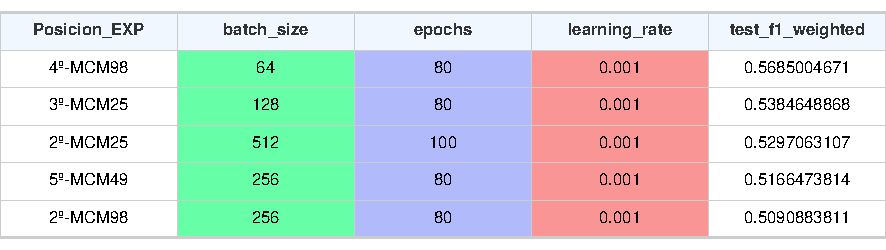
\includegraphics[width=0.9\textwidth]{./img/evaluacion/resultados/top5EVALMCM.pdf}
    \caption{Mejores cinco modelos en la fase de evaluación del modelo de clasificación multiclase.}
    \label{fig:top5EVALMCM}
\end{figure}

